\chapter{深度伪造的对抗性研究與近期研究發展}
\label{chap:4}

本作业在此章节分为三个部分,其一是针对于深度伪造的对抗性部分,这方面则可以从其深度伪造的生成面与检测面来看,其Li XR 等人近期来的汇整工作\cite{2021496} 有可以找到工作成果,另外还有 Yisroel Mirsky 等人 \cite{DBLP:journals/corr/abs-2004-11138} 对其 GAN 的工作总结与近来应用 Transformers 、增量学习在深度伪造领域的检测上的研究工作总结。


\section{深度伪造生成的对抗性}

由于近年来深度伪造技术所生成的人类脸部技术能够轻易修改人类的身分,甚至可以使目标人脸做出想要的脸部肌肉表情,使之在人脸身分辨识的领域遭遇到极大的挑战,同时因应人脸识别的对抗性攻击也不曾间断。其 Goswami G 等人 \cite{goswami2018unravelling},发现基于深度神经网络 (DNN) 架构的模型具有很高的表达能力和学习能力,然而,它们本质上是一种黑盒方法,因为在其多层表示中学习到的函数在数学上表示并不容易。意识到这一点后,许多研究人员已经开始设计方法来利用基于深度学习的演算法的缺点,质疑它们的鲁棒性并暴露它们的奇点。在在此研究中,研究者们试图解开与 DNN 在人脸识别方面的鲁棒性相关的三个方面:(i) 评估深度架构对人脸识别的影响,以应对攻击的脆弱性,这些攻击受到现实世界中普遍观察到的扭曲的启发,浅层学习方法和基于学习的对手可以很好地处理这些扭曲;(ii) 通过表征深层网络隐藏层中的异常滤波器响应行为来检测奇异点;和(iii) 对处理管道进行更正以缓解问题。该研究则使用多个开源的基于 DNN 的人脸识别网络(包括 OpenFace 和 VGG-Face)以及两个公开可用的资料库(MEDS 和 PaSC)的实验评估表明,基于深度学习的人脸识别算法的性能在存在这样的扭曲。同时该方法还与现有的检测算法进行了比较,结果表明,通过使用网络中隐藏层的响应适当地设计分类器,它能够以非常高的精度检测攻击。最后,研究提出了几种有效的对策来减轻对抗性攻击的影响并提高基于 DNN 的人脸识别的整体鲁棒性,其结果发现只要对图片与影像增加一定的遮挡或者在影像加入人类肉眼看不见得噪声,就能够有骗过机器的可能,该工作展示对 Parkhi OM 等人 \cite{parkhi2015deep} 所以提出 VGGface ,与 Baltrušaitis T 等人 \cite{baltruvsaitis2016openface} 所做的 Openface 等模型的实验。

\begin{figure}[htb]
\centering 
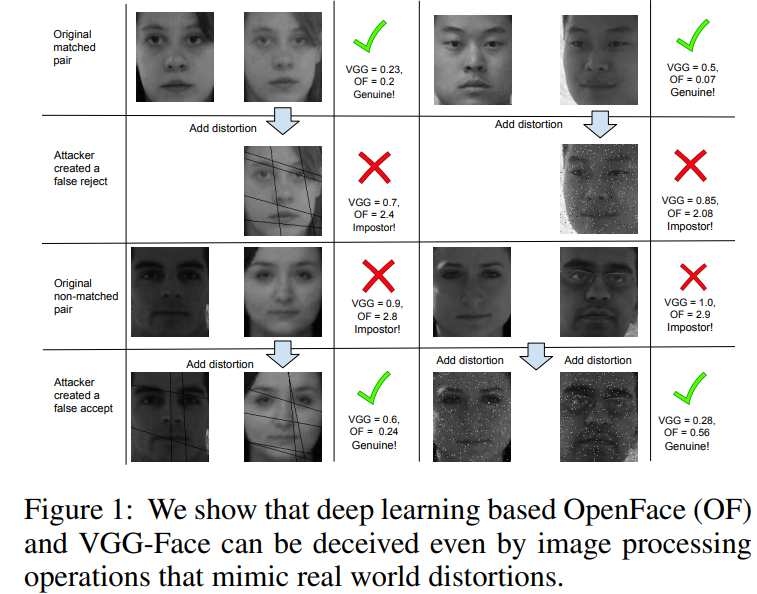
\includegraphics[width=0.90\textwidth]{img/ch4m0.png} 
\caption{ Goswami G 等人 \cite{goswami2018unravelling} }
\label{Test}
\end{figure}

Song Q 等人 \cite{yang2021attacks} 专注于一种对人脸识别网络进行攻击的新颖方法,该方法会误导网络将某人识别为目标人,而不是不明显地错误分类,同时,因为此缘故,研究者引入了一个特定的注意力对抗攻击生成网络来生成假人脸图像。为了捕获目标人的语义信息,这项工作添加了条件变分自动编码器和注意模块来学习人脸之间的实例级对应关系。与传统的双人 GAN 不同,这项工作引入了人脸识别网络作为第三个参与者参与生成器和判别器之间的竞争,这使得攻击者可以更好地模仿目标人。生成的结果难以引起旁观者注意的人脸可以逃避最先进网络的识别,并且大多数人都被识别为目标人。

\begin{figure}[htb]
\centering 
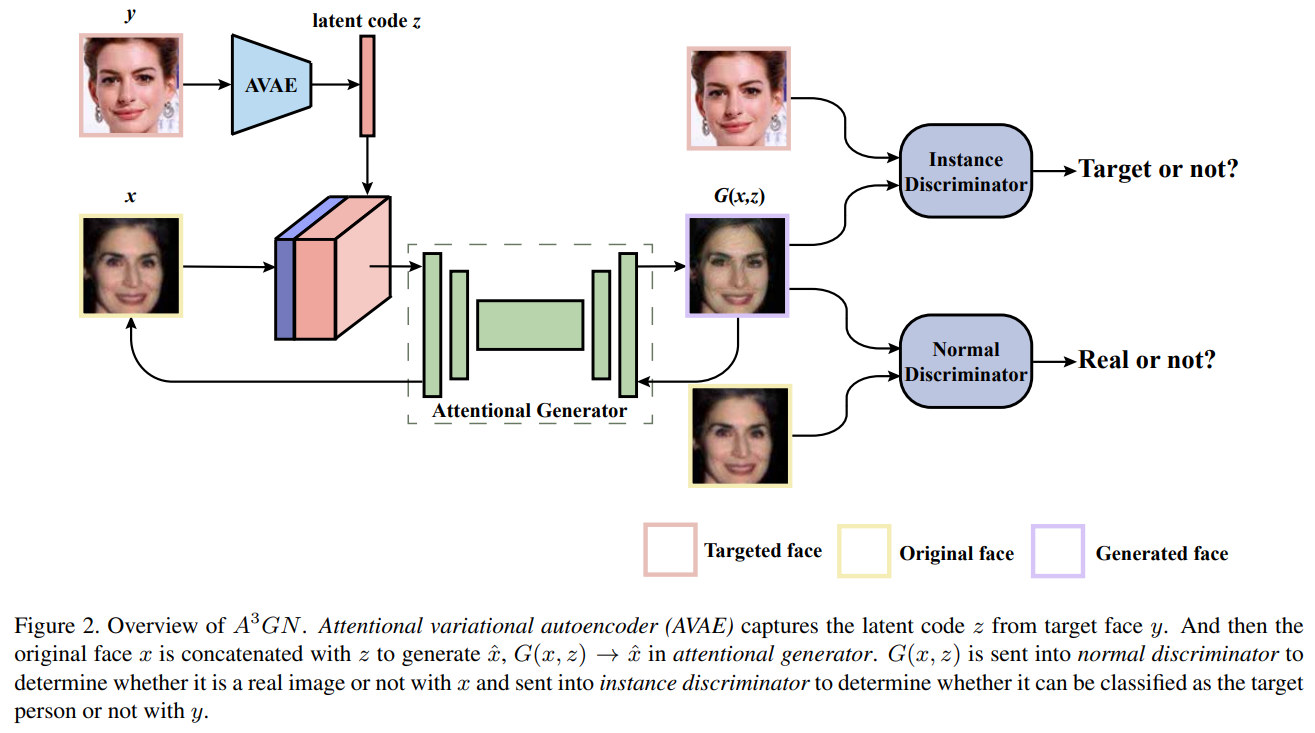
\includegraphics[width=0.90\textwidth]{img/ch4m1.png} 
\caption{ Song Q 等人 \cite{yang2021attacks} }
\label{Test}
\end{figure}

Majumdar P 等人 \cite{majumdar2019evading} 提出了部分面部篡改攻击,其中面部区域被替换或变形以生成篡改样本,而在 CMU-MultiPIE 数据集上使用两个最先进的人脸识别系统 VGG-Face 和 OpenFace 进行的人脸验证实验表明了这些系统对攻击的脆弱性。此外,该研究提出了一种部分人脸篡改检测(PFTD)网络来检测所提出的攻击,该网络通过结合输入图像的原始信息和高频信息来捕获原始图像和篡改图像之间的不一致性,以检测篡改图像。所提出的网络在篡改图像检测方面超越了现有基线深度神经网络的性能。

另外 Korshunov P 等人 \cite{korshunov2018deepfakes},通过使用预先训练的生成对抗网络 (GAN),将视频中的一个人的脸自动替换为另一个人的脸变得越来越容易。最近的公共丑闻,例如,名人的面孔被交换到色情视频上,需要自动检测这些 Deepfake 视频的方法,为了帮助开发此类方法,在本文中,我们展示了第一组从 VidTIMIT 数据库的视频中生成的公开可用的 Deepfake 视频。研究者使用基于 GAN 的开源软件来创建 Deepfakes,该研究强调训练和混合参数可以显著影响结果视频的质量。为了证明这种影响,研究者使用不同调整的参数集生成了具有低和高视觉质量的视频(每个 320 个视频),其研究展示了基于 VGG 和 Facenet 神经网络的最先进的人脸识别系统容易受到 Deepfake 视频的攻击,错误接受率分别为 85.62\% 和 95.00\%,这意味着检测 Deepfake 视频的方法是必要的。通过考虑几种基线方法,我们发现基于口型同步不一致检测的视听方法无法区分 Deepfake 视频。性能最佳的方法,基于视觉质量指标,常用于演示攻击检测领域,在高质量 Deepfakes 上的错误率为 8.97\%,最后的实验表明,GAN 生成的 Deepfake 视频对人脸识别系统和现有检测方法都具有挑战性,而人脸交换技术的进一步发展将使其变得更加困难。同样的也是 Korshunov P 等人 \cite{korshunov2019vulnerability} 展示了 Deepfake 视频的公开数据集,其中的人脸使用基于 GAN 的算法变形,同时为了生成这些影像,研究者使用了基于 GAN 的开源软件,并且我们强调训练和混合参数可以显著影响生成影像的品质,该研究表明,基于 VGG 和 Facenet 神经网络的最先进的人脸识别系统容易受到深度变形视频的影响,错误接受率分别为 85.62 和 95.00,这意味着检测这些视频的方法是必要的。同时研究也考虑了几种检测深度变形的基线方法,并发现基于视觉品质指标的方法(通常用于演示攻击检测领域)导致最佳性能,错误率为 8.97。而最后研究者的实验表明,GAN 生成的深度变形视频对人脸识别系统和现有检测方法都具有挑战性,而深度变形技术的进一步发展将使其更加如此。


\section{深度伪造检测的对抗性}

其深度伪造领域的演算法多数都是运用类神经网路等技术,而其神经网路模型本身即有着对抗样本的攻击,从 Szegedy C 等人 \cite{szegedy2013intriguing} 报告了两个这样的属性。首先,根据单元分析的各种方法,该研究发现单个高级单元和高级单元的随机线性组合之间没有区别。其研究表明,在神经网络的高层中,包含语义信息的是空间,而不是单个单元。其次,研究者们发现深度神经网络学习的输入-输出映射在很大程度上是不连续的。可以通过应用某种不可察觉的扰动来导致网络对图像进行错误分类,这种扰动是通过最大化网络的预测误差来发现的。此外,这些扰动的具体性质并不是学习的随机伪影:相同的扰动可能导致在数据集的不同子集上训练的不同网络对相同的输入进行错误分类。另 Goodfellow IJ 等人 \cite{goodfellow2014explaining} 认为神经网络易受对抗性扰动影响的主要原因是它们的线性性质,这种解释得到了新的定量结果的支持,同时给出了关于它们最有趣的事实的第一个解释:它们在架构和训练集上的泛化。此外,这种观点产生了一种简单而快速的生成对抗样本的方法。使用这种方法为对抗性训练提供示例,该研究减少了 MNIST 数据集上 maxout 网络的测试集误差。

\begin{figure}[htb]
\centering 
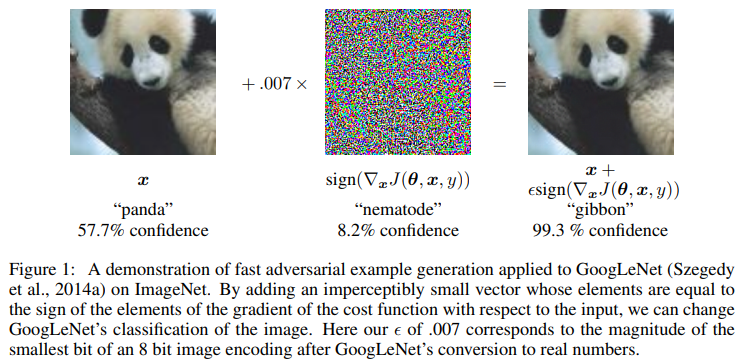
\includegraphics[width=0.90\textwidth]{img/ch4m2.png} 
\caption{ Goodfellow IJ 等人 \cite{goodfellow2014explaining} }
\label{Test}
\end{figure}

另外 Kurakin A 等人 \cite{kurakin2018adversarial} 发现大多数现有的机器学习分类器都非常容易受到对抗性示例的影响,对抗性示例是输入数据的样本,该样本经过了非常轻微的修改,旨在导致机器学习分类器对其进行错误分类。在许多情况下,这些修改可能非常微妙,以至于人类观察者甚至根本没有注意到修改,但分类器仍然会出错。对抗性示例会带来安全问题,因为它们可用于对机器学习系统进行攻击,即使对手无法访问底层模型。到目前为止,所有先前的工作都假设了一个威胁模型,其中攻击者可以将数据直接输入机器学习分类器。在物理世界中运行的系统并非总是如此,例如那些使用来自相机和其他传感器的信号作为输入的系统。该研究表明,即使在这样的物理世界场景中,机器学习系统也容易受到对抗性示例的影响。研究者们通过将从手机摄像头获得的对抗性图像馈送到 ImageNet Inception 分类器并测量系统的分类精度来证明这一点,最后研究者也发现,即使通过摄像头感知,大部分对抗性示例也被错误分类。

从上述几项研究的结果可以得知,这些由神经网络组成的模型在面对对抗性样本攻击时,会导致模型受到干扰,从而产生误判,由此也造成深度伪造技术在生成时可隐藏自身特征,从而绕过检测,由此有必要对当下的模型跟算法做对抗性的评估,另外 Wang SY 等人 \cite{kurakin2018adversarial} 研究尝试是否有可能创造一个“通用”检测器,用于将真实图像与 CNN 生成的图像区分开来,无论使用何种架构或数据集。为了测试这一点,研究者们收集了一个数据集,该数据集由 11 种不同的基于 CNN 的图像生成器模型生成的假图像组成,这些模型跨越当今常用架构的空间(ProGAN、StyleGAN、BigGAN、CycleGAN、StarGAN、GauGAN、DeepFakes、级联细化网络,隐式最大似然估计,二阶注意力超分辨率,在黑暗中看到)。其研究者证明,通过仔细的预处理和后处理以及数据增强,仅在一个特定的 CNN 生成器 (ProGAN) 上训练的标准图像分类器能够很好地泛化到看不见的架构、数据集和训练方法(包括刚刚发布的StyleGAN2)。而研究者的研究结果表明,当今 CNN 生成的图像存在一些常见的系统缺陷,从而阻止它们实现逼真的图像合成,这一有趣的可能性,同时该工作对训练资料进行类似于 JPEG 压缩、模糊等操作手法,可以提高模型的泛化性能。

另外 Neves JC 等人 \cite{neves2020ganprintr} 专注于整个面部图像的合成,这是一种特定类型的面部操作。该研究的主要贡献有四方面:i) 描述了一种从基于自动编码器的合成假图像中去除 GAN“指纹”的新策略,以欺骗面部操作检测系统,同时保持结果图像的视觉质量;ii) 对近期面部操作检测文献的深入分析;iii) 对这种类型的面部操作进行完整的实验评估,考虑到最先进的假检测系统(基于整体深度网络、隐写分析和局部伪影),并指出这项任务在不受约束的场景中的挑战性;最后 iv) 研究者们宣布了一个名为 iFakeFaceDB 的新型公共数据库,该数据库将该研究所提出的 GAN 指纹去除方法 (GANprintR) 应用于已经非常逼真的合成假图像。在该研究的实证评估中获得的结果表明,需要额外的努力来开发针对看不见的条件和欺骗技术的强大的面部操作检测系统,例如本研究中提出的技术。

Brockschmidt J 等人 \cite{brockschmidt2019generality} 
对都属于卷积神经网络 (CNN) 的 Rossler A 等人 \cite{rossler2019faceforensics++} 所做的的 Xception 与 Afchar D 等人 \cite{afchar2018mesonet} 所做的 Mesonet 进行对抗性评估,其实验使用来自六种最先进的面部伪造技术的样本:Deepfakes、Face2Face、FaceSwap、GANnotation、ICface 和 X2Face。研究者发现 MesoNet 和 XceptionNet 显示出泛化到多种欺骗技术的潜力,但在准确性上略有权衡,并且在很大程度上无法对抗看不见的技术。最后将这些结果松散地推断为类似的 CNN 架构,并强调需要更好的架构来应对普遍性的挑战。

Marra F 等人 \cite{marra2018detection} 研究了几种图像伪造检测器对图像到图像转换的性能,无论是在理想条件下,还是在存在压缩的情况下,通常在上传到社交网络时执行。该研究在 36302 张图像的数据集上进行,表明传统和深度学习检测器都可以实现高达 95\% 的检测精度,但只有后者在压缩数据上保持高达 89\% 的高精度,换言之现有的检测器若面对未知的压缩与类型,其表现并不理想。
Zhang X 等人 \cite{zhang2019detecting} 检测 GAN 生成的图像,传统的监督机器学习算法需要从目标 GAN 模型中收集大量真实和虚假图像。但是,攻击者使用的特定模型通常是不可用的。为了解决这个问题,该研究提出了一个 GAN 模拟器 AutoGAN,它可以模拟由几个流行的 GAN 模型共享的公共管道产生的伪影,此外,研究者确定了由通用 GAN 管道中包含的上采样组件引起的独特伪影。该研究从理论上表明,这种伪影表现为频域中光谱的复制,因此提出了一种基于光谱输入而不是像素输入的分类器模型。通过使用模拟图像来训练基于频谱的分类器,即使在训练期间没有看到目标 GAN 模型产生的假图像,此研究的方法在检测由流行 GAN 模型(如 CycleGAN)生成的假图像方面也取得了最先进的性能。

Du M 等人 \cite{du2019towards} 提出了 Locality-Aware AutoEncoder (LAE) 来弥补泛化差距。在训练过程中,研究者使用像素级掩码来规范 LAE 的局部解释,以强制模型从伪造区域学习内在表示,而不是在训练集中捕获伪影并学习表面相关性来执行检测。而该研究进一步提出了一个主动学习框架来选择具有挑战性的标签候选者,该框架需要不到 3\% 的训练数据使用人工蒙版,从而大大减少了规范化解释的注释工作。三个 deepfake 检测任务的实验结果表明,LAE 可以专注于伪造区域来做出决策。分析进一步表明,就先前未见过的操作的泛化精度而言,LAE 在三个深度伪造检测任务上的性能分别优于现有技术 6.52\%、12.03\% 和 3.08\%。

Huang, R 等人 \cite{huang2020security} 通过实验证明了个体对抗性扰动 (IAP) 和普遍对抗性扰动 (UAP) 的存在,它们可能导致表现良好的 FFM 行为不端。基于迭代过程,梯度信息用于生成两种可用于制造分类和分割输出的 IAP。相比之下,UAP 是在过火的基础上生成的。研究者们设计了一个新的目标函数,鼓励神经元过度激发,即使不使用训练数据也可以生成 UAP,实验证明了 UAP 在未见数据集和未见 FFM 之间的可转移性。此外,研究者对对抗性扰动的不可察觉性进行了主观评估,表明精心制作的 UAP 在视觉上可以忽略不计。这些发现为评估 FFM 的对抗性安全性提供了基准。

\section{GAN}

\section{Transformers 與 增量学习}



